%!TEX root = thesis.tex
\chapter{Cryptographic Primitives}
Secure Function Evaluation (SFE) can be split into two cases: cases where there are two parties involved, referred to as two-party computation (2PC), and cases where there are three or more parties, referred to as multiparty computation (MPC).
It turns out that many protocols that work for MPC often don't work for 2PC and vice versa.
This thesis will focus primarily on 2PC protocols, but many of the methods are applicable to MPC as well.

2PC protocols are complex cryptographic protocols that rely on a number of crypographic primitives.
In order to understand 2PC, it is not crucial to understand how the cryptographic primitives work, but it is important to understand their inputs, outputs and security guarantees. 
This first chapter will give an overview of the cryptographic primitives used in 2PC protocols.
\al{stopped here}

\section{Computational Indistinguishability} 
\label{sctn:computational-indistinguishability}

\al{what is computationally Indistinguishability and why is it important?}

\al{set /NN}
Let $\mathcal{X} = \{X(n,a)\}_{n \in \NN, a \in \{0,1\}^*}$ and $\mathcal{Y} = \{Y(n,a)\}_{n \in \NN, a \in \{0,1\}^*}$ be distribution ensembles.
$\mathcal{X}$ and $\mathcal{Y}$ are computationall indistinguishable there is no polynomial-time algorithm that can tell $\mathcal{X}$ and $\mathcal{Y}$ apart with better than neglibible probability.
More formally, $\mathcal{X}$ and $\mathcal{Y}$ are computationally indistinguishable, denoted $\mathcal{X} \compindist \mathcal{Y}$, if and only if for all non-uniform polynomial-time distinguisher $D$, there exists a function $\mu(\cdot)$ that is neglibible in $n$, such that for all $a \in \{0,1\}^*$, 
\begin{equation}
    |Pr[D(X(n,a)) = 1] - Pr[D(Y(n,a)) = 1]| < \mu(n)
\end{equation}
\cite{lindell2009secure}.

\section{Encryption}
Encryption is the process of encoding a message such that only parties with the key can read the message.
As we discuss 2PC, we will be using symmetric-key encryption, the case where encryption and decryption use the same key.
A symmetric-key encryption protocol is composed of two parts.
The first part is the encryption algorithm which obfuscates the message, and the second part is the decryption algorithm which unobfuscates the disguised message.
The encryption algorithm is denoted $\Enc$, and the decyprtion algorithm is denoted as either $\Dec$ or $\EncInv$.
\begin{equation}
    \label{eqn:encryption}
    \begin{split}
        \Enc_k (pt) & = ct  \\
        \Dec_k(pt) = \EncInv_k(ct) & = pt
    \end{split}
\end{equation}
where $pt$ is the original message or the \emph{plaintext}, $ct$ is the encrypted message or the \emph{ciphertext}, and $k$ is the secret key.
For the algorithm to be effective, the secret key $k$ must be a random string of $0$s and $1$s of length $\lambda$.
\footnote{The notion of randomness in cyptoraphy has a precise definition, and in cases where $\lambda$ is large, it is sufficient for $k$ to be pseuodorandom. Pseudorandom also has precise cryptographyic definition.}
$\lambda$ is the security parameter of our protocol.
If we increase $\lambda$, thereby increasing the size of the key, then the encyrption algorithm becomes harder for an adversary to break.
I will not go into details about how encryption algorithms are instantiated; I will merely treat them as algorithms which we can use at our leisure.

We say that encryption scheme is secure \footnote{Specifcally, this is the definition of a chosen-plaintext-attack secure encryption scheme. There exists weaker and stronger definitions of security, but chosen-plaintext-attack security is frequently used for 2PC}, if the following game is true:
\al{give the game and reference computational indistinguishability}

It is useful for 2PC to define a specific type of symmetric-key encryption algorithm called a Dual-Key Cipher (DKC) \cite{bellare2012foundations}.
A DKC requires two secret keys to encrypt and decrypt the message, in constrast to classic encryption which only requires one.
It is easy to instantiate a DKC if one has a secure encryption scheme: let $k_0$ and $k_1$ be the two secret keys and instantiate the DKC as follows:
\begin{equation}
    \begin{split}
        \EncDKC_{k_0, k_1}(pt) = \Enc_{k_1} ( \Enc_{k_0} ( pt )) \\
        \EncDKCInv_{k_0, k_1}(ct) = \EncInv_{k_0} ( \EncInv_{k_1} ( ct )) 
    \end{split}
\end{equation}
This construction of a DKC is slow, and there are many faster methods for instantiating DKCS.
For more information, see \cite{bellare2012foundations}.

\section{Boolean Circuit} 
A function for an 2PC protocol is represented by a boolean circuit.
A boolean circuit takes as input $x \in \{0,1\}^n$ and performs a series of small opreations on the inputs, and outputs a sequence of $y \in \{0,1\}^m$. 
You may have encountered circuits and logical operators in another context, where the inputs and outputs were True and False.
For our usage, True will correspond to the value $1$, and False will corresond to the value $0$. 

The small operations done inside of a circuit are performed by a \emph{gate}.
A gate is composed of three wires: two input wires and one output wire, where a \emph{wire} can have a value either $0$ or $1$.
A gate performs a simpler operation on the two inputs, resulting in a single output bit.
Table \ref{tab:xor} gives the mapping of an XOR gate.
\al{TODO add xor gate}

\begin{table}[h]
\label{tab:xor}
\centering
\begin{tabular}{ | l | c || r |}
\hline
x & y & xor(x,y) \\ \hline
1 & 1 & 0 \\ \hline
1 & 0 & 1 \\ \hline
0 & 1 & 1 \\ \hline
0 & 0 & 0 \\ \hline
\end{tabular}
\caption{The mapping of an XOR gate.}
\end{table}

A circuit is a combination of multiple gates that are stringed together, and it turns out that circuits are quite powerful: in fact, a circuit built out of only AND gates, XOR gates and NOT gates can compute any function or algorithm \al{Find citation}.
In other words, if there's some algorithm that do it, then there is some circuit that can do it as well.
Figure \ref{fig:less_than_circuit} shows the circuit representation of the less than function, $f$ as specified in equation \ref{eqn:less_than}.

\begin{figure}[h]
    \centering
    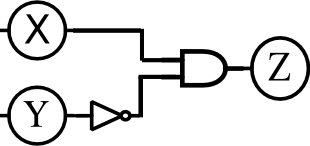
\includegraphics[scale=0.75]{images/drawing.png}
    \label{fig:less_than_circuit}
    \caption{A circuit that computes the less or equal to function, equivalent to $f$ for input of two one-bit values. \al{TODO, add truth table?}}
\end{figure}

\section{Oblivious Transfer}
Oblivious Transfer (OT) is a two-party protocol where one party (sender) has two inputs, $m_0$ and $m_1$, and the other party (receiver) has a bit $b \in \{0,1\}$. 
OT enables the receiver to acquire $m_b$ from the sender without revealing which message was received, i.e. the value of $b$.
Morever, the receiver learned nothing about the message that wasn't received, i.e. anything about $m_{1-b}$.

Here we give the Naor-Pinkas protocol of $1-2$ oblivious transfer.
The protocol relies on the DDH assumption \al{give a source that the reader can check}.

\begin{figure}
    \centering
    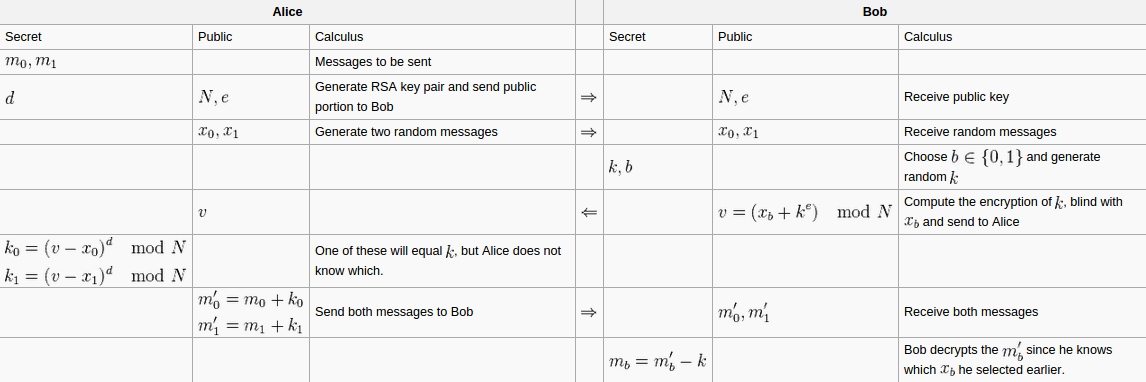
\includegraphics[scale=0.3]{images/ot_wiki}
    \caption{Semi-honest Naor-Pinkas oblivious transfer.}
\end{figure}

Oblivious transfer has been improved in two relevant ways for 2PC protocols. 
These improvments are called OT-extension and OT-preprocessing. 
In OT-extension, a constant number of OT's can be run, to generate a polynomial number of exchanged values.
In OT-preprocessing, the OT's can happen before the actual protocol, during what is called the offline phase, and then when the OT's are needed during the online phase, simpler and efficient communication realizes the exchanged values.
This is useful because the actual OT step requires a large amount of communciation to be sent between the sender and receiver, resulting in OT often being the bottleneck of 2PC protocols.
